\documentclass[a4paper,12pt]{article}
\usepackage{acn-scientific}
\usepackage{acn-questions}

\title{Fraunhofer Alphabet}
\author{\textsc{A.C. Norman}
\\ \texttt{a.norman@olcc.lancs.sch.uk}}
\date{}

%\showanswerstrue
\showanswersfalse

\begin{document}

\thispagestyle{empty}

\maketitle

\vspace*{-0.3cm}

\noindent Based on \emph{Fraunhofer Alphabet} Alan Winter 1980 \emph{Phys. Educ.} \textbf{15} 291

\enlargethispage{3cm}

\begin{itemize}
\item The patterns below show the diffraction patterns of capital letters. 
\item The patterns are in alphabetical  order.
\item There are 22 (out of 26 possible) patterns; four letters are missing.
\end{itemize}

\begin{enumerate}
    \item Which are the four missing letters?
    \item Sketch what you expect each of the missing diffraction patterns to look like.
\end{enumerate}

\thispagestyle{empty}

\begin{center}
    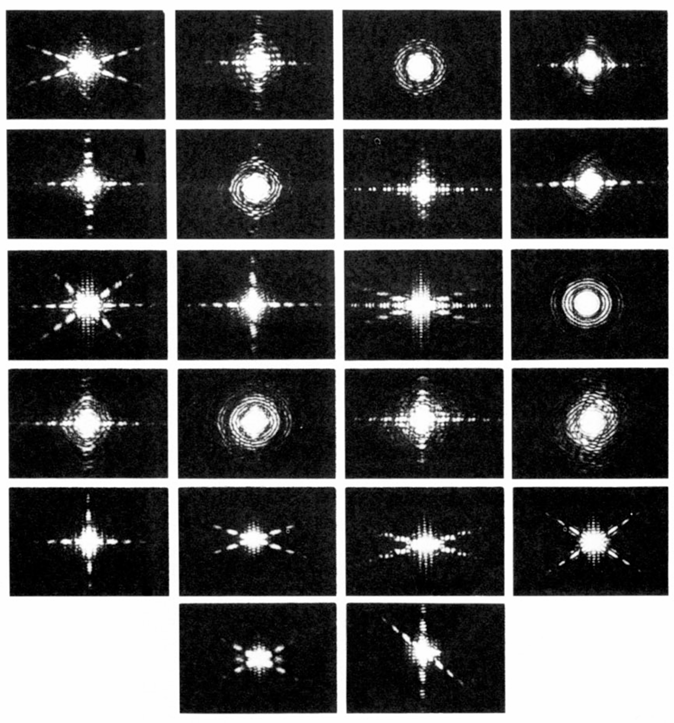
\includegraphics[width=\textwidth]{img/Winter1980-patterns.png}
\end{center}

%\vfill
%\ccbyncsa
\end{document}